\section{Aplicația de redare}

Obiectele shader reprezintă codul GLSL compilat pentru o singură etapă shader. Acestea pot fi create folosind funcția $glCreateShader$ ce primește ca parametru tipul de shader ce trebuie creat printr-un enum, cele mai comune valori pentru acesta fiind $GL\_VERTEX\_SHADER$ și $GL\_FRAGMENT\_SHADER$ \cite{openglreference}. Prin această valoare este specificată pentru ce etapa este stocat codul din shader. Odată creat obiectul shader în acesta trebuie stocat codul sursă GLSL. Acest lucru poate fi făcut cu funcția $glShaderSource$, care primește că parametru o listă de șiruri de caractere \cite{openglreference}. Când shader-ul este compilat, acesta va fi compilat ca și cum toate șirurile date ar fi concatenate. Odată ce șirurile de caractere ce reprezintă codul sursă pentru un shader au fost stocate într-un obiect shader, acesta poate fi compilat cu funcția $glCompileShader$. Compilarea shaderului poate eșua, iar pentru aceasta trebuie verificată valoarea $GL\_COMPILE\_STATUS$ din obiectul shader \cite{openglreference}. În cazul în care aceasta indică faptul că a existat o eroare în procesul de compilare, eroarea poate fi identificată cu ajutorul funcției $glGetShaderInfoLog$. Atunci când au fost create toate obiectele shader necesare acestea trebuie link-editate într-un program. În această etapă pot există erori, și acestea pot fi tratate în același mod că în etapa de compilare, singura diferență fiind verificarea valorii $GL\_LINK\_STATUS$ în loc de $GL\_COMPILE\_STATUS$ \cite{openglreference}.

Shader vertex este etapa Shader programabilă din pipeline-ul de redare care se ocupă de procesarea nodurilor individuale. Un vertex shader primește un singur vârf din fluxul de vârf și generează un singur vârf în fluxul de vârf de ieșire. Trebuie să existe o corespondență 1:1 de la vârfurile de intrare la vârfurile de ieșire. În această aplicație acest shader este folosit pentru a transforma pozițiile vârfurilor din spațiu local în spațiul camerei. Shaderul vertex folosit este cel din anexa \hyperref[appendix:16_raycasting_vert]{16}.

Matricea modelului $M$ este compusă din transformarea de translație $T$ a unui obiect, transformarea de rotație $R$ și transformarea de scalare $S$. Înmulțirea poziției unui vertex $v$ cu această matrice model transformă vectorul în spațiul global \cite{LearnOpenGL}.

\begin{equation}
    M = T \cdot R \cdot S
\end{equation}
\begin{equation}
    v_{world} = M \cdot v_{model}
\end{equation}

Camera are, de asemenea, o matrice model care definește poziția sa în spațiul global. Inversul matricei modelului camerei $V$ este matricea de vizualizare și transformă vârfurile din spațiul global în spațiul camerei sau spațiul de vizualizare.
Odată ce vârfurile sunt în spațiul camerei, ele pot fi transformate în spațiul clip prin aplicarea unei transformări de proiecție. Matricea de proiecție $P$ codifică cât de mult din scenă este surprinsă într-o redare prin definirea marginilor vizualizării camerei. Cele mai comune două tipuri de proiecție sunt perspectivă și ortografică. Proiecția în perspectivă are ca rezultat efectul natural al lucrurilor care par mai mici cu cât sunt mai departe de privitor \cite{LearnOpenGL}. 

Poziția finală a vârfurilor este obținută după ecuația:

\begin{equation}
    v_{final} = P \cdot V \cdot M \cdot v 
\end{equation}

Un shader fragment este etapa shader care va procesa un fragment generat de rasterizare într-un set de culori și o singură valoare de adâncime. Shaderul de fragmente este etapa pipeline-ului OpenGL după ce o primitivă este rasterizată. Pentru fiecare eșantion de pixeli acoperiți de o primitivă, este generat un fragment, fiecare dintre acestea are o poziție în spațiul ferestrei de vizualizare și conține toate valorile de ieșire interpolate pentru fiecare vârf din ultima etapă de procesare vertex. Ieșirea unui fragment shader este o valoare de adâncime și mai multe valori de culoare care pot fi scrise în buffer-urile din framebuffer-urile curente. Fragment shaders iau un singur fragment ca intrare și produc un singur fragment ca ieșire \cite{LearnOpenGL}. 

Shaderul de fragmente este folosit pentru a aplica tehnica ray casting specifică afișării datelor volumetrice. Acest algoritm este compus din 4 etape pentru fiecare pixel:

\begin{enumerate}
    \item Este calculată intersecția volumului cu o rază ce are originea în pixel și este perpendiculară pe suprafața ecranului.
    \item Este realizată eșantionarea volumului în puncte echidistante de-a lungul razei ce se află în interiorul casetei de încadrare.
    \item Se obține valoarea funcției de transfer pe baza valorii intensității în punct.
    \item Toate proprietățile optice rezultate sunt acumulate rezultând culoarea și opacitatea finală a pixelului.
\end{enumerate}

Punctele de origine ale razelor sunt invariante la rotația și scalarea obiectului, dar acestea trebuie modificate atunci când sunt efectuate operații de translație asupra acestuia. Shaderul de fragmente utilizat pentru ray casting este în anexa \hyperref[appendix:17_raycasting_frag]{17} Opacitatea finală a fiecărui fragment depinde de rata de eșantionare. Aceasta poate fi corectată folosind formula:

\begin{equation}
    A=1-(1-A)^\frac{s_0}{s},
\end{equation}
unde $A$ este valoarea opactiatii punctului curent, $s$ este rata de eșantionare folosită și $s_0$ este o rată de eșantionare de referință. Aceasta este utilizată pentru corectarea opacității funcției de transfer ori de câte ori utilizatorul modifică rata de eșantionare $s$ de la rata de eșantionare de referință $s_0$ \cite{gpugems39}.

\begin{figure}[!h]
    \centering
    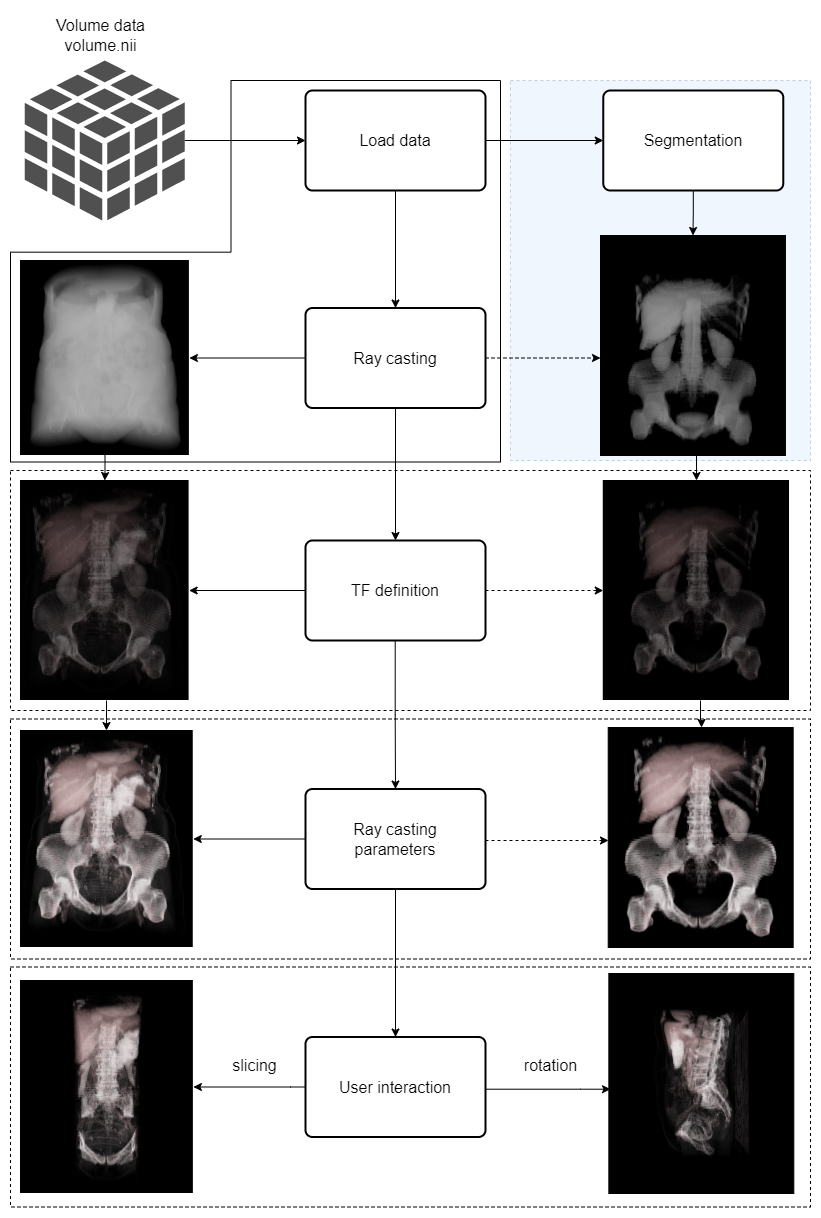
\includegraphics[width=14cm]{images/licenta_io_diagram.png}
    \\
    \caption{Diagrama etapelor procesului de redare a unei imagini volumetrice. După fiecare etapă redarea poate fi îmbunătățită de către utilizator prin definirea unei funcții de transfer, optimizarea parametrilor folosiți de ray casting sau prin generarea și aplicarea măștii de segmentare.}
    \label{fig:app_diagram}
\end{figure}

În figura \ref{fig:app_diagram} este prezentat procesul de creere a unei redări semnificative a unui volum. Etapele ce sunt încadrate în dreptunghiuri cu linie punctată sunt opționale, sau pot fi realizate în altă ordine decât cea prezentată. În partea din dreapta este prezentat rezultatul aplicării măștii de segmentare peste rezultatul obținut în imaginea din stânga pentru aceeași etapă. Segmentarea poate fi generată sau încărcată din memorie în cazul în care a mai fost generată, sau există o segmentare manuală disponibilă. În momentul încărcării unui alt volum masca de segmentare este reinițializată, dar funcțiile de transfer și valorile parametrilor pentru ray casting rămân stocate în aplicație. Modalitatea de alterare a funcției de transfer și parametrii ce pot fi ajustați pentru vizualizare sunt prezentate în secțiunea următoare.


\begin{figure}[!h]
    \centering
    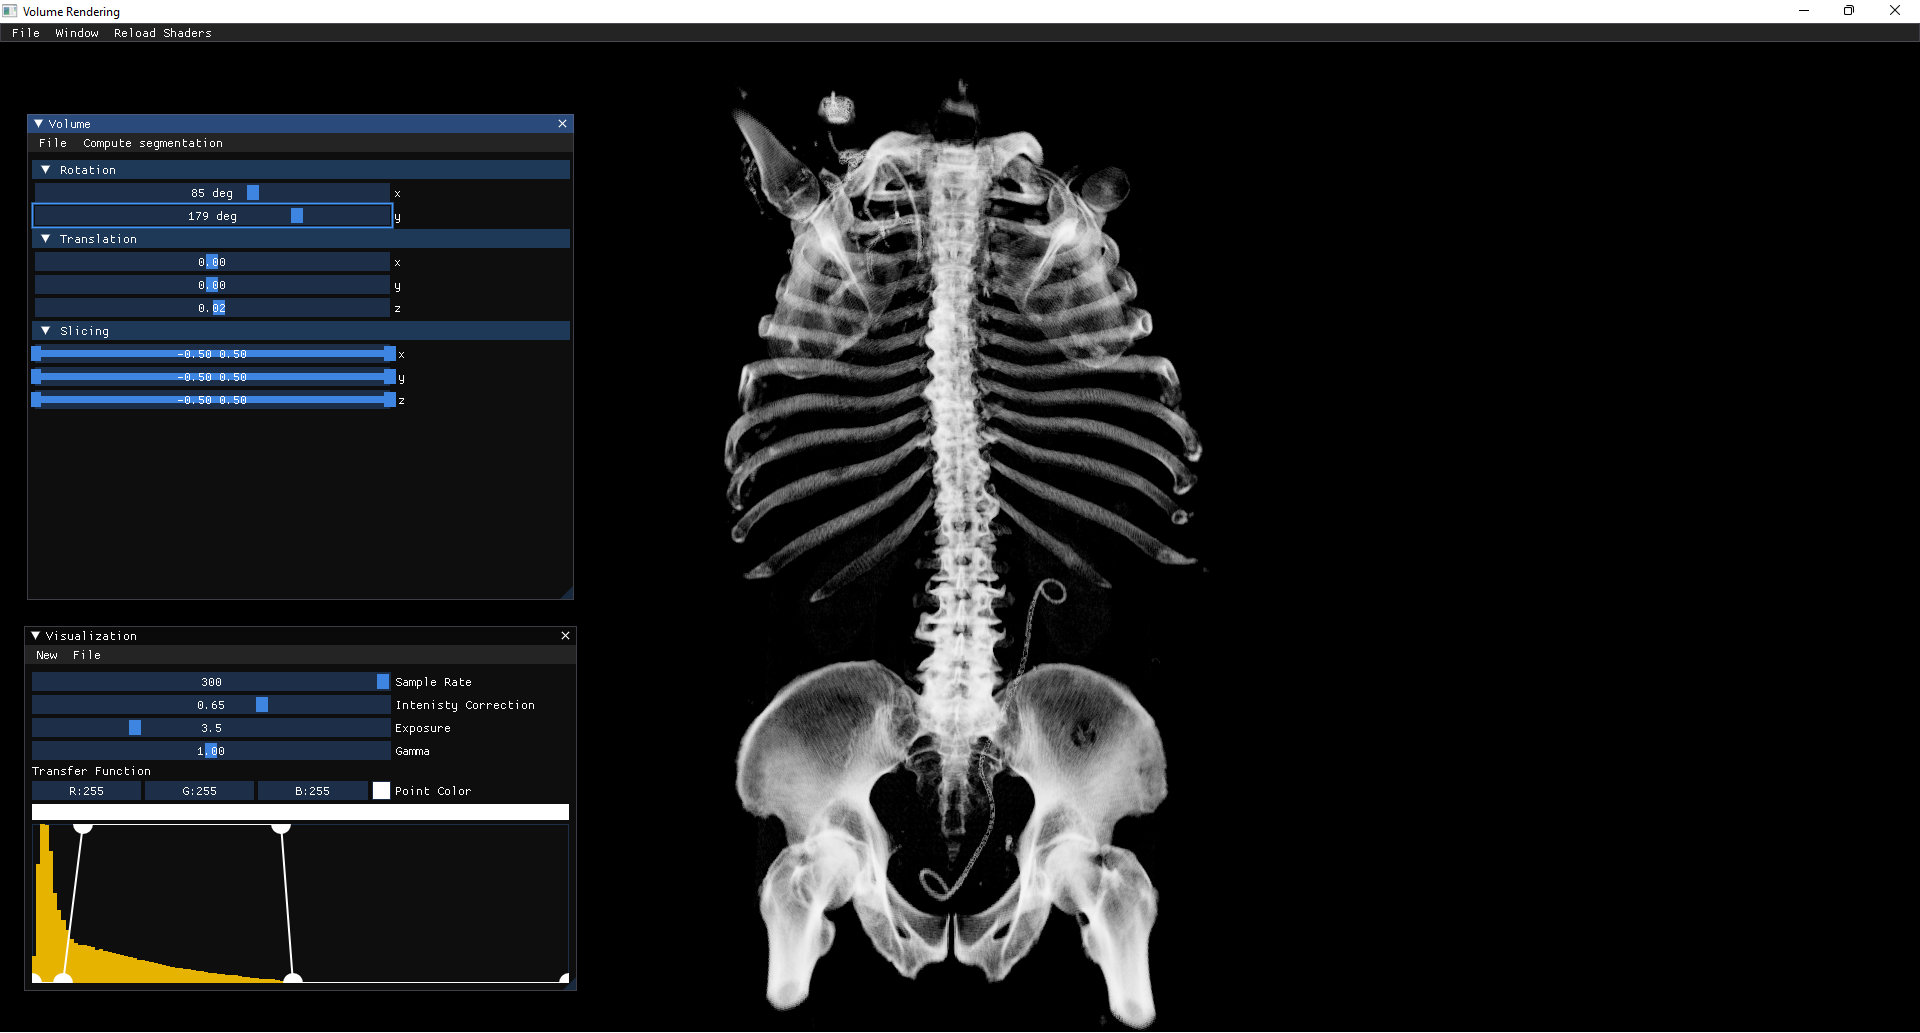
\includegraphics[width=15cm]{images/prt_app.png}
    \\
    \caption{Exemplu de vizualizare a unei imagini volumetrice în aplicația C++. A fost creată o funcție de transfer astfel încât să fie evidențiată structura osoasă a pacientului.}
    \label{fig:viz_volume}
\end{figure}

\begin{figure}[!h]
    \centering
    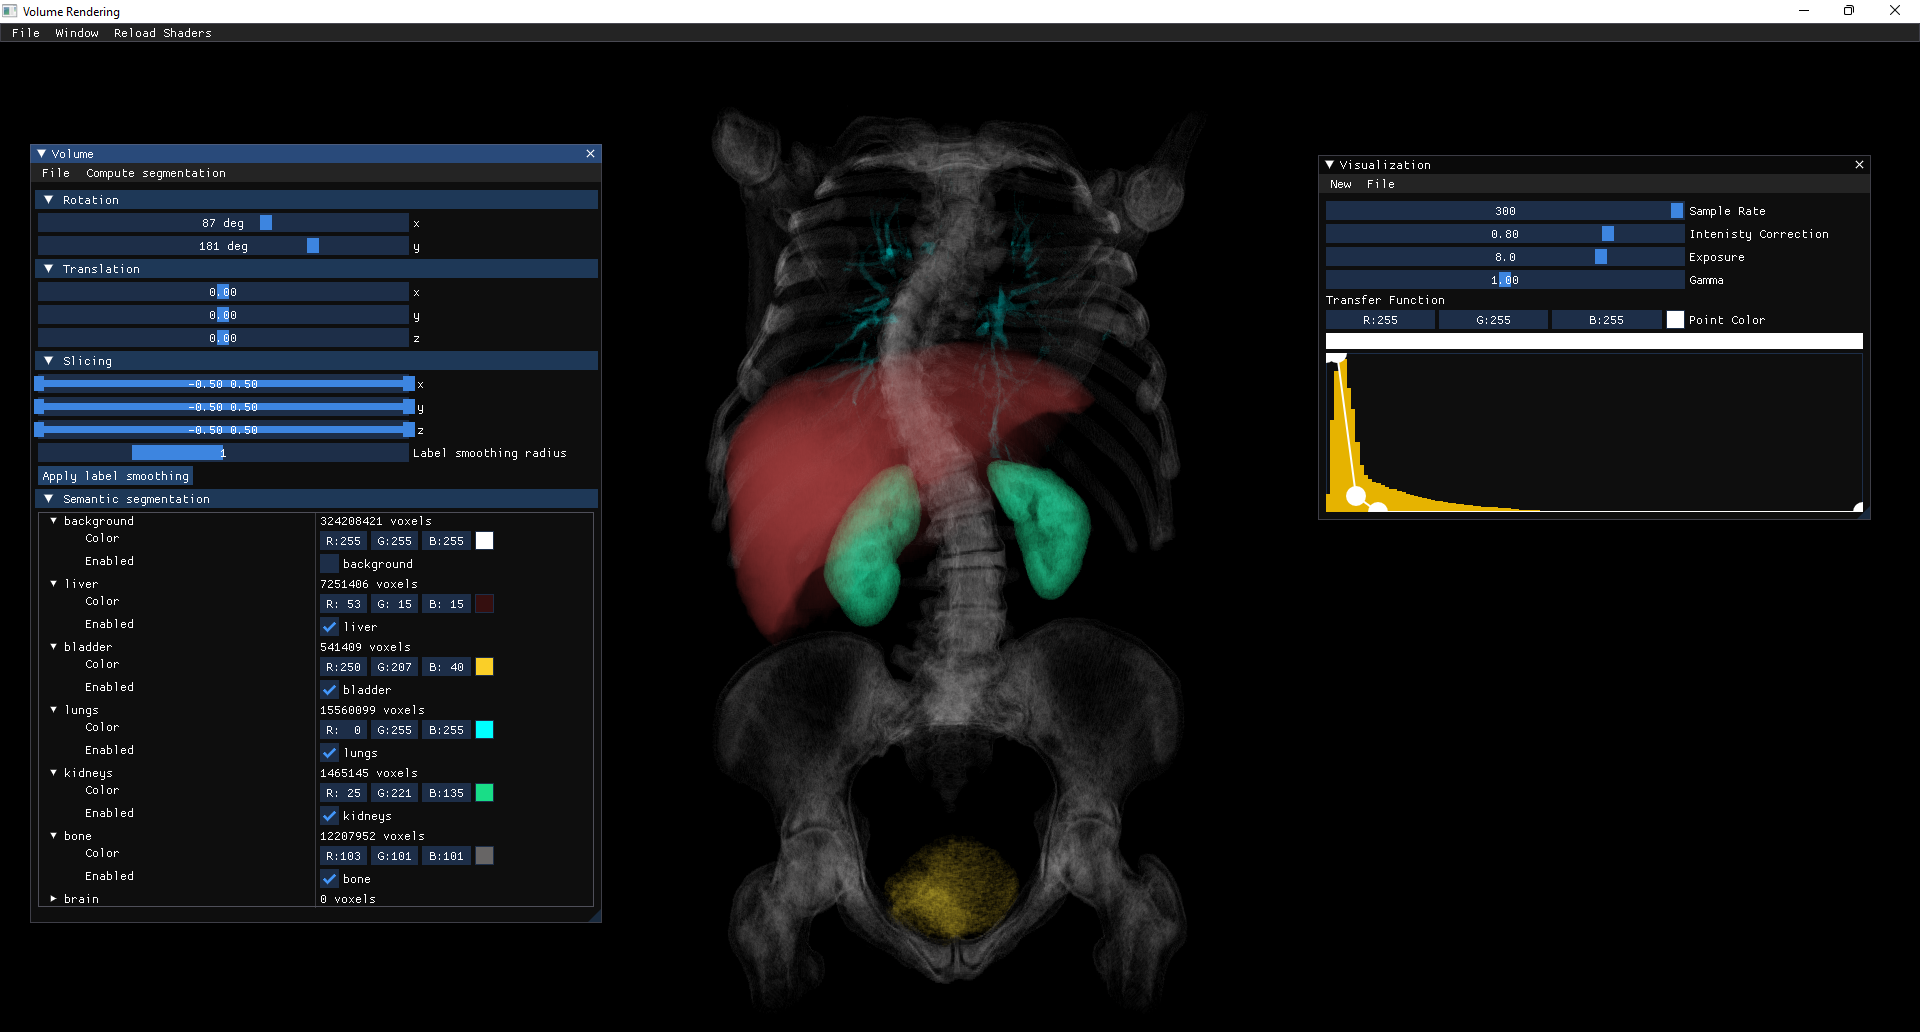
\includegraphics[width=15cm]{images/prt_app_seg.png}
    \\
    \caption{Îmbunătățirea vizualizării folosind segmentarea semantică. Fiecare tip de regiune din masca de segmentare are atribuită o culoare diferită pentru evidențiere.}
    \label{fig:viz_volume_seg}
\end{figure}

În figura \ref{fig:viz_volume} se regăsește o captură de ecran a aplicației atunci când a fost încărcat un volum de înaltă calitate și a fost aleasă o funcție de transfer care să evidențieze structura osoasă a pacientului. În acest, folosind widget-ul pentru crearea funcției de transfer, a fost creată o formă trapezoidală, astfel funcția atribuie voxelilor cu intensitate scăzută (reprezentând țesuturi moi precum organe, piele, mushi etc.) opacitate 0. Pentru intensitățile mai mari decât maximul existent în volumul reprezentant nu este importantă forma funcției de transfer, deoarece nu afectează redarea. În figura \ref{fig:viz_volume_seg} se regăsește, de asemenea, o captură de ecran a aplicației în care a fost folosită o mască de segmentare pentru îmbunătățirea vizualizării. Fiecare etichetă are atribuită o culoare diferită pentru evidențierea diferitelor clase de segmentare.


\section{Interfața cu utilizatorul}

Dear ImGui este o bibliotecă C++ pentru interfață grafică cu utilizatorul minimalistă, fară dependențe externe. Este necesar un backend pentru a integra Dear ImGui în aplicație care transmite intrări de la periferice și este responsabil de redarea buffer-urilor rezultate. Sunt furnizate backend-uri pentru o varietate de API-uri grafice și platforme de redare, de interes fiind în special cel pentru GLUT. ImGui crează interfețe bazate pe ferestre ce pot fi redimensionate și plasate oriunde în fereastra aplicației. Poziția și dimenisunile ferestrelor sunt stocate într-un fișier de configurare, care în mod implicit este denumit "imgui.ini". În acest fișier vor fi stocate, folosind funcții noi după modelul celor existente pentru ferestre, culori pentru elementele din interfață, marcaje pentru browser-ul de fișiere și parametrii pentru modelul de segmentare.


\begin{figure}[!h]
    \centering
    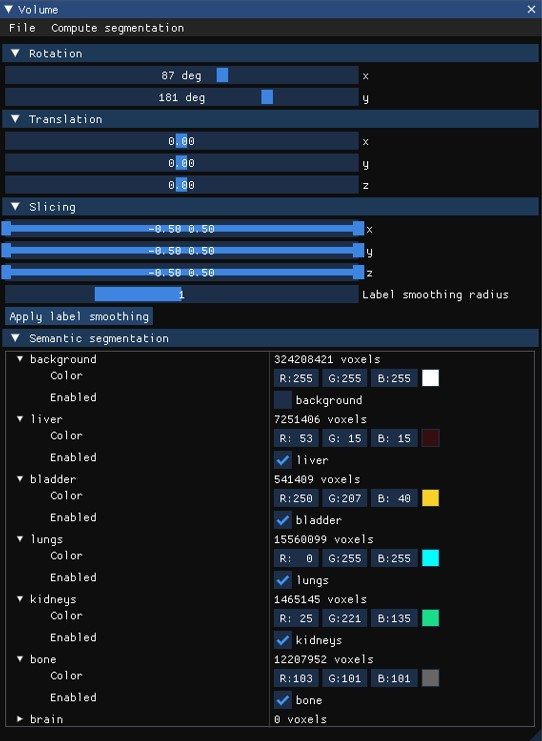
\includegraphics[width=12cm]{images/wnd_vol.jpg}
    \\
    \caption{Fereastra din care pot fi manipulate perspectiva vizualizării volumului și regiunile vizibile cu ajutorul măștii de segmentare.}
    \label{fig:viz_volume_wnd}
\end{figure}

În figura \ref{fig:viz_volume_wnd} este o captură de ecran a ferestrei "Volume" din aplicația de vizualizare. Această fereastră este împărțită în patru regiuni ce pot fi restrânse:
\begin{enumerate}
    \item "Rotation" - în această porțiune a ferestrei sunt două slidere care arată și manipulează unghiul din care este vizualizat volumul, pe două axe. Vizualizarea din diferite unghiuri este importantă deoarece este prezentat un obiect tridimensional într-o imagine 2D, asfel sunt pierdute multe detalii într-o singura redare, fiind necesare multiple redări din diferite unghiuri pentru redarea întregului volum.
    \item "Translation" - sunt prezente trei slidere care manipulează și prezintă locația în spatiu a volumului pe cele trei axe. Acestea sunt utile atunci când este aplicat zoom asupra volumului, astfel fiind vizibilă doar regiunea centrală. În acest caz, pentru vizualizarea cu zoom a regiunilor mai apropiate de marginile volumului, este necesară aplicarea unei translări spațiale a cubului în care se realizează redarea. O altă utilitate a operației de translare este aceea de a permite amplasarea ferestrelor interfeței în fereastra aplicației și mutarea cubului volumului astfel încât acesta să fie vizibil.
    \item "Semantic segmentation" - în această regiune a ferestrei este împărțită într-un tabel cu șapte rânduri, unul pentru fiecare clasă de segmentare și doua coloane, în stânga fiind eticheta clasei de segmentare și în dreapta numărul de voxeli care aparțin acelei etichete. Fiecare rând poate de descoperit pentru a afișa încă două rânduri în care se regăsește un selector de culoare pentru clasa respectivă, și un \textit{toggle} care controlează dacă regiunile marcate cu eticheta respectivă sunt sau nu redate.
\end{enumerate}


\begin{figure}[!h]
    \centering
    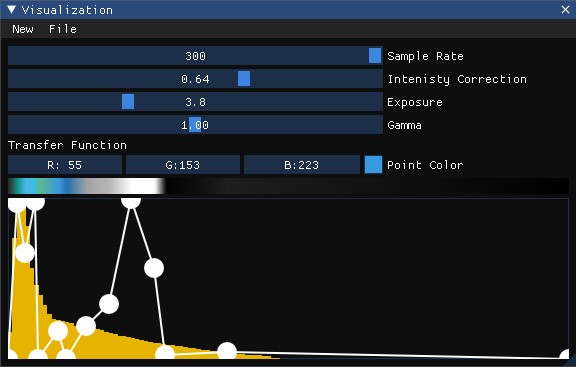
\includegraphics[width=12cm]{images/wnd_tf.jpg}
    \\
    \caption{Fereastra din care pot fi modificate funcția de transfer și valorile specifice vizualizării.}
    \label{fig:viz_tf_wnd}
\end{figure}

În figura \ref{fig:viz_tf_wnd} este o captură de ecran a ferestrei în care pot fi schimbate aspecte legate de vizualizarea modelului. Întâi sunt afișate patru slidere care modifică valori ce afectează rezultatul redării.

\begin{enumerate}
    \item "Sample Rate" reprezintă rata de eșantionare, adică în câte puncte echidistante sunt preluate intensități din volum pentru compunerea lor pentru obținerea rezultatului redării.
    \item "Intensity Correction" este valoarea cu care este înmulțită intensitatea la ficeare pas din etapa de compunere.
    \item "Exposure" este folosit pentru modificarea intensității rezultatului obținut după etapa de compunere.
    \item "Gamma" este valoarea folosită pentru corecția gamma.
\end{enumerate}

În partea de jos a acestei ferestre este un widget care permite creerea unei funcțîi de transfer liniare prin amplasarea punctelor într-un grafic. Distanța punctelor fată de axa Ox reprezintă valoarea transparenței. Punctele pot fi adăugate, șterse și repozitionate cu ajutorul mouse-ul. Atunci când este selectat un punct, acestuia îi poate fi atribuită o culoare. Rezultatul poate fi previzualizat în partea de sus a graficului. Funcția de transfer care este trimisă către obiectul shader este obținută prin interpolare liniară pentru puncte și culorile lor atribuite. Graficul funcției de transfer este peste o histogramă a intensităților volumului curent, pentru a ajuta utilizatorul în creerea unei funcții de transfer relevante.

\begin{figure}[!h]
    \centering
    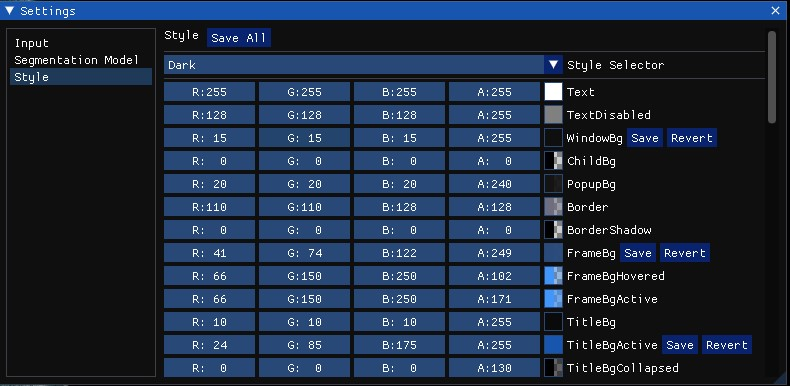
\includegraphics[width=12cm]{images/wnd_settings.jpg}
    \\
    \caption{Fereastra în care pot fi schimbate setările aplicației.}
    \label{fig:viz_settings_wnd}
\end{figure}

ImGui facilitează modificarea culorilor din interfața cu utilizatorul, așadar în fereastra "Settngs" prezentată în figura \ref{fig:viz_settings_wnd} există un tab în care sunt înșirate toate culorile ce pot fi schimbate, iar schimbările care sunt făcute pot fi salvate. Pe lângă acesta, mai există două tab-uri: unul în care pot fi schimbate vitezele cu care se rotește sau translează volumul, și celălalt conține parametrii necesari pentru funcționarea modelului de segmentare semantică (dimensiunea la care va fi redimensionat volumul înainte ca acesta să fie dat ca intrare la rețeaua neuronală).
